%
% $Id: SANDtemplate.tex,v 1.3 2007-12-13 21:27:14 rolf Exp $
% A template to build SAND reports. See the examples for more details and
% formatting suggestions. A command reference is available at
% http://www.cs.sandia.gov/~rolf/SANDreport
%
\documentclass[pdf,12pt,report,strict]{SANDreport}
\usepackage{comment}
\usepackage{verbatim,xspace,url,graphicx,subfigure,times}
\usepackage{listings}
\usepackage[section]{placeins}
\lstset{language=C++,basicstyle={\ttfamily\scriptsize},breaklines,breakatwhitespace}


%\newcommand{\eph}{Ephemeris\xspace}
%\newcommand{\Eph}{Ephemeris\xspace}

% ---------------------------------------------------------------------------- %
% Set the title, author, and date
%
    \title{Flexible and Scalable Data Fusion using Proactive, Schemaless Information Services}
    \author{Patrick M. Widener\\Scalable System Software Department\\Sandia National
      Laboratories\\P.O. Box 5800\\Albuquerque, NM 87185-1319}		% Use First, Middle, Initial
    \date{}		% Leave this here but empty


% ---------------------------------------------------------------------------- %
% These are mandatory
%
\SANDnum{SAND2014-16250}		% e.g. \SANDnum{SAND2006-0420}
\SANDprintDate{June 2014}	% Month, year
\SANDauthor{Patrick M. Widener}		% One line, separated by commas


% ---------------------------------------------------------------------------- %
% These are optional
%
%\SANDrePrintDate{}	% May be repeated for successive printings
%\SANDsupersed{}{}	% {Old SAND number}{Old date}


% ---------------------------------------------------------------------------- %
% Build your markings. See example files and SAND Report Guide
%
    %\SANDreleaseType{}
    %\SANDmarkTopBottomCoverBackTitle{}
    %\SANDmarkBottomCover{}
    %\SANDmarkTopBottomCoverTitle{}
    %\SANDmarkTop{}
    %\SANDmarkBottom{}
    %\SANDmarkTopBottom{}
    %\SANDmarkCover{}
    %\SANDmarkCoverTitle{}


% ---------------------------------------------------------------------------- %
% Start the document
%
\begin{document}
    \maketitle

    % ------------------------------------------------------------------------ %
    % An Abstract is required for SAND reports
    %
    \begin{abstract}
Exascale data environments are fast approaching, driven by diverse structured and unstructured data such
as system and application telemetry streams, open-source information capture, and on-demand simulation
output. Storage costs having plummeted, the question is now one of converting vast stores of data to
actionable information. Complicating this problem are the low degrees of awareness across domain
boundaries about what potentially useful data may exist, and write-once-read-never issues (data
generation/collection rates outpacing data analysis and integration rates). Increasingly, technologists
and researchers need to correlate previously unrelated data sources and artifacts to produce fused data
views for domain-specific purposes. New tools and approaches for creating such views from vast amounts of
data are vitally important to maintaining research and operational momentum. We propose to research and develop tools and services to assist in the creation, refinement, discovery and reuse of fused data views over large, diverse collections of heterogeneously structured data. We innovate in the following ways. First, we enable and encourage end-users to introduce customized index methods selected for local benefit rather than for global interaction (flexible multi-indexing). We envision rich combinations of such views on application data: views that span backing stores with different semantics, that introduce analytic methods of indexing, and that define multiple views on individual data items. We specifically decline to “build a big fused database of everything” providing a centralized index over all data, or to export a rigid schema to all comers as in federated query approaches. Second, we proactively advertise these application-specific views so that they may be programmatically reused and extended (data proactivity). Through this mechanism, both changes in state (new data in existing view collected) and changes in structure (new or derived view exists) are made known. Lastly, we embrace “found data heterogeneity” by coupling multi-indexing to backing stores with appropriate semantics (as opposed to a single store or schema).
     \end{abstract}


    % ------------------------------------------------------------------------ %
    % An Acknowledgment section is optional but important
    %
    \clearpage
    \chapter*{Acknowledgments}
This work was funded under LDRD Project Number 164869 and Title ``Flexible and Scalable Data Fusion using
Proactive, Schemaless Information Services''.

The following individuals have given me valuable feedback and assistance during the project documented by
this report: Travis Bauer, Ann Campbell, Warren Davis, Bill Hart, Thomas Kroeger, and Judy Spomer.

    % ------------------------------------------------------------------------ %
    % The table of contents and list of figures and tables
    %
    \cleardoublepage		% TOC needs to start on an odd page
    \tableofcontents
    \listoffigures
    \listoftables

\begin{comment}
    % ---------------------------------------------------------------------- %
    % An optional preface or Foreword
    \clearpage
    \chapter*{Preface}
    \addcontentsline{toc}{chapter}{Preface}


    % ---------------------------------------------------------------------- %
    % An optional executive summary
    \clearpage
    \chapter*{Summary}
    \addcontentsline{toc}{chapter}{Summary}


    % ---------------------------------------------------------------------- %
    % An optional glossary. We don't want it to be numbered
    \clearpage
    \chapter*{Nomenclature}
    \addcontentsline{toc}{chapter}{Nomenclature}
    \begin{description}
	\item[Term 1]
	    Description
	\item[Term 2]
	    Description
	\item[Term 3]
	    Description
    \end{description}
\end{comment}

    % ---------------------------------------------------------------------- %
    % This is where the body of the report begins; usually with an Introduction
    %
    \SANDmain		% Start the main part of the report

    \section{Introduction and Background}

This report discusses the background, design, and implementation of a software service, Drift, designed to
support \emph{data fusion}.  We use the term to mean the ability to treat distinct, possibly
heterogeneous, pieces of data as a single entity, for the purposes of identification, manipulation, and
analysis.  We address a universe of structured and semi-structured data, from scientific experimental and
simulation results and inputs about which almost all possible metadata is known to word-processor and
spreadsheet documents whose provenance is unclear.  

Indeed, this disparity in metadata availability in large part motivates this project.  An abstract data
type (ADT) is a idiom directly supported by object-oriented programming languages, in which developers
are encouraged to map the intellectual process of data-driven design from the top (i.e. the ``real
world'') down, as opposed to trying to think in detail about varied collections of primitive data types.
Drift represents an exploration of applying this principle at a higher level.  Fast networks, cheap
near-line storage, and the emergence of ``big data'' problems have led engineers and
scientists to develop data-centric design and problem-solving processes.  These processes incorporate many different kinds
of data produced by different methods, with varying degrees of attached metadata, and with lifetimes
exceeding typical project durations or even employee tenures.  

Drift explores the possibility of forming abstractions around data that has no previous explicit
interrelationships.  We see much of the potential usefulness of a service such as Drift in assisting
users to make explicit relationships between data that were previously part of shared understanding, 
cultural assumptions, or hand-me-down knowledge among developers, or artificially separated by
administrative or other boundaries.  Making these relationships 
explicit and available has the potential to reduce misconceptions about how data in organizations is
used.  

Although making it easier to define such abstractions, to fuse data, is a key goal of Drift, it is also
an enabling step for data analysis.  Assigning names to fused data objects is one way to reference them,
but applying analytic techniques to that naming process promises interesting benefits.  In particular,
using components of the fused data itself to drive indexing schemes that support automated learning and
categorization can provide important leverage for queries and data mining-style operations.  In this
Drift is designed to support making fused data objects into ``first-class'' entities for the purposes of
data mining and analysis, to be operated on using analytic methods in the same way as primitive data
types are in current usage.


\subsection{Background and approach}

The database research community was among the first to address problems of data fusion, exploring
approaches such as revised relational algebras and SQL optimization\cite{bleiholder09:_data}. Large-scale availability of
distributed system middleware later drove investigations into federated database and query
services\cite{busse99:_feder_infor_system,sheth90:_feder} in 3-tier enterprise application architectures,
and this flavor of data fusion has persisted through an evolution to service-oriented
architectures\cite{papazoglou03:_servic}.

Drift is intended to improve the availability and utility of federated query-style data services for
researchers in large-data environments comprising multiple heterogeneous sources by making it easier for
them to construct views on distributed data that are meaningful to them. Drift embodies a proposition
that significant expressive power can be obtained by connecting application-specific views to fused and
discrete data sources (flexible multi-indexing), and that tools and software systems that directly
support this will prove useful. Drift's design further assumes that, given such tools and systems,
facilities that provide push-based notification of changes in those views and that can be integrated
directly into applications and data (data proactivity) will also prove useful.

Our method of defining and advertising views on distributed data is more flexible than traditional
federated query approaches in that it encourages a “bottom-up” approach where multiple, perhaps
inconsistent views on the same data are possible. Rather than finding ways to limit the proliferation of
these views, Drift makes them reusable and extensible. Drift also aims to reintroduce distributed query
capabilities for data other than semantically organized text, as much recent research has emphasized
federated text search\cite{sparql}. In contrast to existing data mining/analysis tools such as
Splunk\cite{splunk}, Drift provides programmatic solutions compatible with extremely high-throughput
streaming data environments where indexing, analysis and shaping of metadata and data must be performed
\emph{in situ}, and where advanced analytic indexing capabilities can be introduced directly by scientists and
researchers.


By implementing flexible multi-indexing, Drift enables users to define their own customized views for the
metadata they are concerned with, and directly embed these structures into a metadata service. While
defining indexing structures is a fairly straightforward (and obviously useful) operation for commonly
used hierarchical naming structures such as tries, we believe that more novel results will come from the
use of analytic data structures for indexing. 

For example, as high-dimensional, “big-data” scenarios become commonplace, and in a dynamic metadata
environment such as that we envision, kd-trees\cite{bentley80:_multid} whose dimensional components can
be customized by end-users have the potential to provide extremely granular data selection while still
maintaining efficient indexing. Another example is the use of a kd-tree to implement a nearest-neighbor
search, which can for example complement the automatic classification tasks in the Cyber domain. Of
particular interest are scenarios where metadata objects (potentially comprising multiple objects
spanning multiple backing data stores) can be indexed by more than one user-defined index structure (for
example, consider a feature set generated by computational simulation, indexed both hierarchically by a
trie and by an N- dimensional hyperplane through the feature set).

Users wishing to construct a new fused data product through the use of multiple indexes may wish to know
if related data products are already available so that those products might be reused or extended. Drift
provides a publish/subscribe-like model where entities interested in changes in the data represented in a
service, or changes in the structure of the service itself (addition of new indexes, for example), can be
proactively notified rather than having to interrogate the service.  This style of state management
provides an asynchronous, eventually-consistent global picture of the available views defined by all
users, which is both necessary to enable discovery and encourage reuse, and more flexible and scalable
than federated query approaches enforcing stricter consistency semantics. We also expect proactivity to
provide direct benefits to users, allowing coupling between computational or sensor-based
results. Consider for example the advertisement of a fused data product that must await a cooperating
computation to be completed, or the establishment of a condition driven by asynchronous external
phenomena (such as a malicious network attack detected by a stateful firewall). Proactive interfaces can
also complement the trigger- or change-based mechanisms already available in the backing stores Drift
uses.

Drift uses flexible and scalable schemaless data stores to store and make available
heterogeneously-structured and unstructured data. These tools have been studied in detail at Sandia and
elsewhere, and Drift does not innovate in their design or construction. There are several flavors of
these stores, each representing a particular choice of trade-offs: key-value (Amazon
Dynamo\cite{Hastorun07dynamo:amazons} and descendants), column-oriented (e.g. Google
BigTable\cite{Chang06bigtable:a}, Apache Cassandra), document-oriented (e.g. Couch, Mongo), and
graph/RDF/adjacency (e.g. Neo4j, Allegro). Drift uses this diversity of data representation to more
effectively cope with the variety of data and metadata we expect to encounter.

More interestingly, Drift extends traditional federated-query-style data management by providing the
ability to construct logical views over physical data residing in multiple such stores, leveraging the
unique benefits of each. For example, the best method for representing relationships between documents
might be a graph database, but it could prove useful to associate that relationship with sets of
experimental results residing in a column-store. Lastly, being able to incorporate tools like HBase
(thereby coupling map-reduce computations) enables a further degree of richness in data view definition.

\subsection{Use Cases}

Issues raised in the following use cases motivate our work:

\begin{enumerate}
\item Long-running engineering efforts accumulate vast stores of different but equally important data
  over time as artifacts of design, testing, and production.  Design documents include reports,
  schematics, spreadsheets, emails, and other notes; these are typically produced by and manipulated with
  commercial office productivity software such as Microsoft Office.  Testing data adds to this large
  amounts of numerical results, test descriptions, and parameter sets.  Production data adds another type
  of data store to the problem, as database management software is frequently used to maintain inventory
  information.  When problems are detected during testing or production use, answering the questions that
  lead to root causes requires a holistic look back at a large and interrelated data space: What testing
  regime was used for the widget in question?  was its design valid?  how many of these widgets are in
  production?  Combining different heterogeneous data in the right ways can quickly illuminate these
  issues.

\item Certain corporate data must be mined for features which are relevant to ongoing operations.  For
  instance, streaming telemetry collection from internal cloud deployments can pose issues deriving from
  all four of the ``V's'' of big data: volume, velocity, variety, and veracity.  This telemetry can
  include system health and performance monitoring as well as application data streams.  Fusing these
  data streams to support enterprise decision-making is an important capability (consider, for example,
  an internal cloud-based ``honeypot'' used to isolate, diagnose, and respond to cybersecurity attacks in
  near-real-time).
\end{enumerate}



%%% Local Variables: 
%%% mode: latex
%%% TeX-master: "paper"
%%% End: 


    \newcommand{\driftd}{\texttt{driftd}\xspace}
\newcommand{\libdrift}{\texttt{libdrift}\xspace}
\newcommand{\dpart}{\texttt{Part}\xspace}
\newcommand{\dparts}{\texttt{Part}s\xspace}

\section{The Drift Service}

\emph{Drift} is a client/server implementation, based on publish/subscribe middleware, of the data fusion
service design described in the previous section.  The following components of Drift are of interest and
will be discussed in more detail in this chapter.

\begin{itemize}
\item A persistent daemon \texttt{driftd} that runs as an independent process on a POSIX-flavored system;
\item A client library, \libdrift, of C++ objects that are used to interact with \driftd;
\item An instance of the Neo4J graph database, used by \driftd for relationship management;
\item An (optional) instance of the MongoDB schemaless data store, used by \driftd for arbitrary data
  storage;
\item An (optional) instance of the Mule Enterprise Service Bus, whose integration with Drift is
  described in Chapter~\ref{sec:ephemeris}.
\end{itemize}

\section{\driftd}

\driftd is a persistent, independent process which receives messages from clients and sends response
messages to those clients.  \driftd also periodically sends advertisement messages with certain
information about the current state of the service as well as update messages when information items
managed by the service undergo state changes.  These advertisement and proactive messages go out to any
interested (\emph{subscribed}) party.  

\driftd encapsulates several capabilities and/or subsystems of note which will be described in this
chapter. All communication is accomplished in a \emph{publish/subscribe messaging} style and is enabled by a
third-party messaging subsystem.  This subsystem also provides the infrastructure for defining message
types and is responsible for data marshaling between client and server.  \emph{Flexible analytic
  indexing} provides novel ways for clients to refer to data items.  The \emph{raison d'\^{e}tre} of
Drift is its implementation of \emph{data fusion}, which is accomplished via a composite data structure
termed the \emph{parts list}.  Finally, we discuss the \emph{proactivity} features of Drift and how they
make interacting with the service more natural.

\subsection{Publish/subscribe messaging}

Drift is based in part on ideas realized in a research artifact known as the \emph{Proactive Directory
  Service}\cite{bustamante02:_scalab_direc_servic_using_proac}.  This service was used as a key
infrastructure component for several years, but over time several shortcomings were identified.  In
particular, PDS required clients to establish a session-based conversation with a server using a set of
remote procedure calls (RPCs). Clients that were only interested in updates about data items or otherwise
had limited or bursty interactions with the server were forced to maintain this session for the duration
of their interaction.  Part of the design rationale for PDS was to provide a more lightweight,
scalable means of information awareness among cooperating processes.  Even though this situation only
affected a certain subset of applications using PDS, this was enough to justify revisiting the design.

Interactions with \driftd are explicitly message-based, as opposed to RPC-based, and there is no notion
of a persistent session with a particular instance of \driftd. A publish/subscribe (pub/sub) model is implemented,
and while \driftd is a central point of published messages, there is in principle nothing preventing
multiple \driftd services from operating cooperatively in a peer-to-peer arrangement.  The implementation
described here assumes a single \driftd instance.

There are many implementations of pub/sub middleware available as open-source software, each with
relative advantages and disadvantages.  We now describe the EVpath middleware that was chosen for the
implementation of Drift.

\subsubsection{EVpath middleware}

EVpath\cite{eisenhauer09:_event} is an event transport middleware layer that can be used to form
arbitrary dataflow graphs among cooperating processes.  EVpath is built around the concept of
\emph{stones} (as in ``stepping stones'') which can be linked together to form a path.  Stones in EVpath
are lightweight entities that roughly correspond to processing points in dataflow diagrams.  Stones of
different types perform data filtering, data transformation, mux and demux of data as well as
transmission of data between processes over network links.  

\begin{figure}
  \center{
    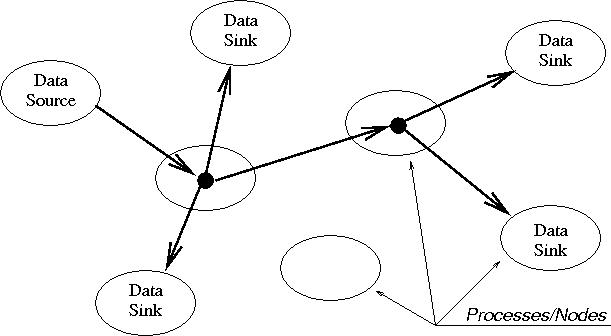
\includegraphics[width=5in]{figs/overlay.jpg}
    \caption{An example dataflow network that can be implemented using EVpath.}
  }
  \label{fig:evpath-overlay}
\end{figure}

Figure~\ref{fig:evpath-overlay} shows an example dataflow network that one might use EVpath to
implement.  Connected stones distribute data from the source through the network to the sinks.  It's
unreasonable to assume that all sinks are interested in the same data, and in fact each sink might want
to customize the event stream in its own particular way (with sink $i$ customizing its stream with a
function $F_i$).  An efficient implementation of event delivery would place these \emph{filter} functions
as close to the source as possible to avoid transmitting unwanted data that would only be discarded on
arrival at its destination (Figure~\ref{fig:evpath-func1}).

\begin{figure}
    \center{
      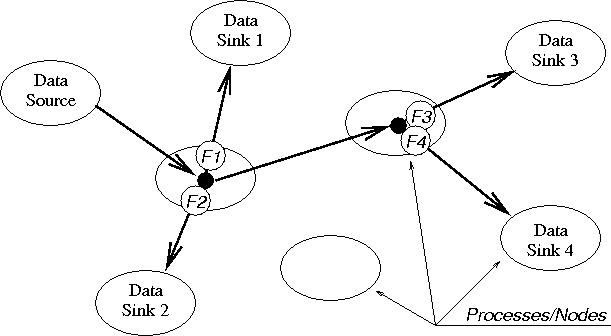
\includegraphics[width=5in]{figs/func1.jpg}
      \caption{A customized dataflow network that can be implemented with EVpath.}
    }
    \label{fig:evpath-func1}
\end{figure}

Drift uses EVpath to establish just such dataflow graphs between \driftd and its clients.  Furthermore,
Drift allows clients using \libdrift to customize their event streams (this is described more fully in
Section~\ref{sec:proactivity}. 

\subsubsection{Constructing messages}

Part of EVpath's management of the dataflow graph is the marshaling and unmarshaling of data as it is
passed to and from the network.  EVpath relies on a companion library, FFS~\cite{eisenhauer11:FFS}, to
accomplish the message definition and description required for this data management.  Drift, in turn,
uses FFS facilities to define the different messages that are exchanged between \driftd and its clients.

\begin{figure}
\begin{lstlisting}
typedef struct _simple_part_xfer {
    unsigned long flags;
    struct _simple_part part;
    char* index_name;
    char* index_spec;
  } simple_part_xfer, *simple_part_xfer_ptr;


FMField drift::simple_part_xfer_fields[] =
    {
      {"flags", "integer", sizeof(unsigned long), FMOffset(drift::simple_part_xfer_ptr, flags)},
      {"part", "simple_part", sizeof(drift::simple_part), FMOffset(drift::simple_part_xfer_ptr, part)},
      {"index_name", "string", sizeof(char*), FMOffset(drift::simple_part_xfer_ptr, index_name)},
      {"index_spec", "string", sizeof(char*), FMOffset(drift::simple_part_xfer_ptr, index_spec)},
      FMfields_terminator
    };
\end{lstlisting}
\label{fig:field-list}
\end{figure}

Figure~\ref{fig:field-list} shows how a sample Drift message is defined using FFS for use with EVpath.
The message structures are defined in conventional C-language style for use in the code of clients and
\driftd, but extra information has to be supplied in order for those structures to be marshaled to and
from the network.  An exhaustive description of all the message definition options possible in FFS is
beyond the scope of this document, but examining this structure in slightly more detail is instructive:

Each field of the C structure is represented in a metadata structure used by FFS.  Each field is tagged
with the following:
\begin{itemize}
\item A type specifier (e.g. ``integer'' for \texttt{flags}).  This specifier indicates what kind of
  marshaling is required for the field, which can enable certain optimizations.  This corresponds loosely
  to C-style typing but size and signed-ness is not reflected here.
\item The size of the field in bytes.
\item The offset of the field from the beginning of the structure.
\end{itemize}

New messages are added to the set that \driftd understands by defining them in this fashion.  While
recompilation is necessary to incorporate new messages defined using this method, there are also some
limited EVpath facilities for defining message types dynamically and using introspection-based
marshaling.  


\subsubsection{Processing messages in \driftd}

All defined messages are registered by \driftd with EVpath and given an associated handler function.
These handler functions are called asynchronously when messages arrive.  Each handler has access to the
main Drift service object in \driftd, and uses this object reference to invoke methods on the service
object.  The body of \driftd is simply an event loop, waiting on messages to arrive and their handler
functions to use the service object.  Appropriate thread exclusion measures are used by \driftd to ensure
the integrity of its internal data.

\newcommand{\partclass}{\texttt{drift::part}}

\subsection{Data Fusion, Relationship Management, and the Parts List}


Drift's data fusion functionality revolves around the \dpart concept.  Fundamentally, a
\dpart encapsulates the following:
\begin{itemize}
\item A datum, along with any metadata necessary to store or retrieve that datum;
\item A UUID that can be associated with index entries in any index maintained by a \driftd instance;
\item A list of ``child'' \dparts
\end{itemize}
In this section we describe how \dparts are used by \driftd to store and retrieve data, the different
types of data storage used by \driftd, and how relationships between fused \dparts are maintained.

\subsubsection{How \dparts operate}

The \dpart concept is realized in a class, \partclass.  This class encapsulates the information
described above.  Each time \driftd receives a request to associate a datum with an index entry, it
generates an UUID (using the \texttt{boost::uuid} library).  These UUIDs are formed in part using the
network address of the service and so are designed to be globally unique across multiple \driftd
instances.  The UUID is then added as the stored value, using the given indexing information in the
request, to the specified index structure.  It is important to note that \dparts know nothing about the
various index structures maintained by \driftd \textemdash they cannot retrieve the index key of any
entries they may be associated with.

Drift allows more than one index to maintain an entry associated with a particular UUID.  This allows
very flexible treatment of data items.  For instance, enumerating a complete set of data items using a
name-based index is straightforward, and it might be useful to simultaneously be able to perform
nearest-neighbor searches on members of that set (based on information maintained in another index
structure).  

\subsubsection{Data storage}

Once a UUID is associated with a \partclass instance, the metadata for the indicated datum is handled.
\driftd distinguishes between two types of storage for data, \emph{immediate} and \emph{external}.  This
reflects a need to compromise between efficiency and flexibility.  Many uses of Drift will involve simple
or primitive data items \textemdash character strings and real or integral numbers.  Rather than generate
metadata and store these primitive items in MongoDB, \driftd denotes the \dpart holding that data as
\emph{immediate} and loads/stores the data along with the \dpart metadata.  In practice, this means that
immediate data items are kept in the memory of the \driftd process, and accessing them does not typically
require a request to an external database.  While there are caching issues associated with this type of
behavior, addressing them is not a priority for Drift.  

An \emph{external} data item has associated with it sufficient metadata to store and retrieve it from
some backing store external to the \driftd process.  \driftd makes use of its companion MongoDB database
for some external items, and for these the metadata consists of the database, collection, and column name
sets required to uniquely identify data within a MongoDB service.  Other external data can include items
in relational databases, for which the metadata contains database connection information as well as a SQL
query that will retrieve the data.  Another external type is files on a filesystem, for which the
metadata is a Universal Resource Locator (URL) that can be used to retrieve the file from a remote
location.  

\partclass has methods for loading and storing data from the storage specified by the metadata.  There is
currently a size threshold beyond which a \dpart's data will not be held by \driftd in memory, and any
requests for it will be satisfied by forwarding the current metadata to the requestor.  

\subsubsection{Relationship management}

A \dpart also contains the foundations for data fusion.  This is implemented in each \partclass by an
associative set of \emph{child} \dpart references and UUIDs.  Constructing a fused data part is then done
internally to \driftd by adding a set of child \dparts to this set.  The fused \dpart, being an instance
of \partclass, is given a UUID and can be indexed just like any other.  From the user point of view,
since \dparts are not typically referred to by UUID (although there is a message type that will send the
UUID on \driftd's advertisement channel), a set of index entries representing different \dparts is
supplied as part of a ``fuse'' request along with a proposed index entry to refer to the fused \dpart.

\dpart metadata on the backing store indicates whether the \dpart is a fused part or not.  If so, the set
of child \dpart UUIDs is retrieved and each \dpart's data is loaded in turn as though it were a simple
\dpart.  While nothing in principle prevents this recursive design from extending to arbitrary levels of
\dpart composition, the current \driftd implementation prohibits \dparts that are part of a composite
from holding child \dparts themselves.

In order to persist information about \dpart relationships, Drift uses the Neo4j~\footnote{Available at
  \url{http://www.neo4j.org/}.} graph database. This information could have been stored using
MongoDB or a low-overhead relational database like SQLlite.  The choice of using Neo4j as opposed to
SQLlite came down to a design tradeoff.  SQLlite functions as an in-memory query-able data store
with persistence ability, while Neo4j requires a connection to an external process.  It was decided that
the more natural representation of a network of interrelated \dparts would be obtained by using Neo4j,
which would not require the multiple joins of a relational database solution or the relatively
complicated query expressions needed to store and retrieve that representation in a column-store like
Mongo.  Additionally, this choice gives \driftd greater control over its own memory usage, allowing it to
trade greater request latency for a smaller footprint; for an asynchronously-oriented service this seems
a reasonable choice.

A composite \dpart with 5 child \dparts in its part-list is persisted in Neo4j as a \dpart node with
outgoing arcs to 5 other \dpart nodes.  The Neo4j API allows information about all such related nodes to
be retrieved with a single call to the server, which is convenient for \driftd's purposes.
Neo4j allows the association of data with relationship entities (conceptually, associating data with arcs
in the relationship graph).  \dpart UUIDS, metadata, and immediate \dpart values are stored in these
property lists.  For \dparts that are not immediate-data, or those whose immediate data values exceed the
size threshold, the metadata for retrieving that data from MongoDB is stored instead (in MongoDB these
data are stored as a column-set indexed by UUID).  

\driftd communicates with the Neo4j server using a REST-style interface over HTTP.  There is no C/C++
language level interface for Neo4j, and even in other development languages the language-level libraries
are implemented on top of Neo4j's REST interface.  We use the open-source
Casablanca REST SDK~\footnote{Available at \url{http://casablanca.codeplex.com/}.} to facilitate
communication through the REST APIs of Neo4j and other services~\footnote{Incidentally, it is our use of
  Casablanca which drives the requirement of a C++ compiler implementing the C++-11 standard in order to
  build \driftd.}.  Load and store operations of \dparts are implemented by calling through the
Casablanca library to Neo4j.  


\subsection{Flexible Analytic Indexing}

Flexible analytic indexing is central to the design of Drift.  \emph{Flexible} refers to the ability of
\driftd to accommodate user-defined data structures into its architecture without requiring major code
changes.  Two of the three existing indexes used by \driftd are \emph{analytic} ones, allowing arbitrary
data to be tracked using selected features either from the data itself or selected by the user.  This
section describes the three index structures used by \driftd and discusses possible future enhancements
to the indexing arrangement.

\subsubsection{Prefix trie}

A hierarchical name space is a basic means of organizing information.  File systems, the Windows
registry, and several directory service protocols have all provided such name spaces; they are
well-understood and highly flexible.  The base data structure for these name spaces tends to be
associative data structures with character strings for keys; very frequently some form of hash table is
chosen.  


\begin{figure}
  \center{
    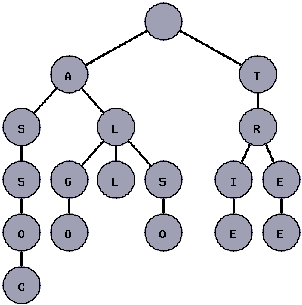
\includegraphics[width=3in]{figs/alg_tries}
    \caption{An example of a prefix tree.}
  }
  \label{fig:trie}
\end{figure}

Another associative structure that can be used for this, and the one that Drift uses, is a
\emph{prefix trie} or \emph{trie}\cite{briandais59:_file}.  Tries have lookup-cost and storage advantages
over hash tables, especially when the entire trie can fit in memory.  A \driftd instance contains a
\texttt{Trie} class object that is used to implement a POSIX-style hierarchical mapping of '/'-delimited
strings to UUIDs.  This is intended to be the default index structure for Drift, and should prove to be
sufficient for many application needs.



\subsubsection{R-tree and kd-tree}

A large part of the utility of Drift comes from its ability to use analytic methods to map to
\texttt{Parts}.  Indexes that deal with multidimensional data, in particular, are useful for ``big data''
applications.  Two such indexes are the \emph{kd-tree}\cite{bentley80:_multid} and
\emph{R-tree}\cite{gutman84:_r,beckmann90:_r}.  

\begin{figure}
  \center{
    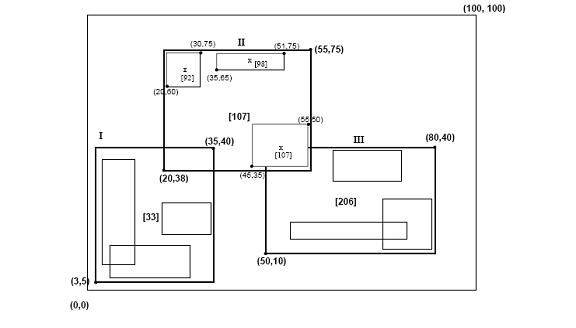
\includegraphics[width=5in]{figs/data-rects}
    \caption{Visualization of data layout in an R-tree.}
  }
  \label{fig:r-tree}
\end{figure}

A kd-tree is useful for splitting a $k$-dimensional search
space into hyperplanes, in the same way a binary tree partitions its key space into two halves at each
node.  A kd-tree is a generalization of a binary tree for data with $k$ dimensions.  The kd-tree is
useful for efficient range-based and nearest-neighbor searches of multidimensional data.  

R-trees are used primarily for spatial indexing of multi-dimensional data.  Where a kd-tree would, by
construction, split each dimension in the key space into halves at each node of the tree, an R-tree
organizes its key space hierarchically, in that each node in the tree forms a ``bounding polygon'' that
``contains'' the keys in the subtree beneath it.  R-trees are generally used to index geographical data
and polygons for graphical systems, and Drift's usage of them is analogous.  To illustrate, consider
using an R-tree to index machines in a data center using a vector of performance data from each machine
as the key space.  An R-tree would then allow the identification of a set of machines contained in a
range for each component of that vector (identifying the minimum bounding polygon where each point in the
polygon is represented by a component of the vector).  This is a slightly different but related query and
result than would be handled by a kd-tree.  For instance, a nearest-neighbor query of a kd-tree would
return only the nearest $N$ neighbors, even if there were $2N$ neighbors in the given range; the R-tree
would return all the neighbors in the ranges specified in the query.

The current \driftd implementation uses an R-tree implementation provided by the Boost suite of C++
libraries\cite{boost_c_librar_spatial_index}.  The kd-tree implementation is an open-source library\cite{krafft}.


\subsubsection{Discussion}

We recognize that the index structures included with Drift are unlikely to address all possible indexing
needs.  This is a key design aspect of Drift realized in the \dpart concept.  Any associative container
that can map some input to a \dpart will be sufficient for Drift, as long as a set of message definitions
and handlers are added to allow \libdrift clients to use it.

Drift was originally designed to accommodate index addition at runtime.  This design goal was eventually
deferred in order to achieve a sort of ``minimum viable implementation'' which could be used as a basis
for iteration and improvement.  However, future possible extensions to Drift may revisit this issue.

Currently, adding an additional index to Drift requires modification of the project source and
rebuilding.  More flexible options were considered as part of the design, each with tradeoffs between
ease of programming, deployment, and performance.  The first is the use of a C++ shared object containing
the new index structures and message definitions.  Installing a new index is triggered by a message from
a client with a reference to the shared object, which is loaded using the\texttt{dlopen()} system call.
This obviously requires shared objects for all possible desired indexes to be deployed along with
\driftd.  

The second solution relies on a C++-to-Python passthrough, where new index structures can be moved
between address spaces running Python interpeters using that languages built-in code mobility
facilities.  Access to the \dpart UUIDs maintained by \libdrift is accomplished through a specialized set
of messages.  This approach, with at least one interposed layer of software, imposes additional
performance penalties, although in Drift's intended usage regimes it's unclear that this would be a
practical issue.

Other more radical rearchitectures of Drift to solve this issue are possible, and were considered during
the design stage.  One in particular would implement the entire indexing layer in Python, communicating
with a separate UUID/\dpart management service.  

Another interesting question for possible future evolution of Drift is which indexes might be useful to
incorporate as first-class citizens, as it were, by bundling them in the source code.  Possibly of
greatest interest here is the use of remote processing to point to a \dpart.  In this way, significantly
more complex analysis on multi-dimensional data might be possible, at the cost of extra network traffic.
Such architectures are common in enterprise systems, where output from multiple application logic tiers
is combined in order to produce a logically-organized response to an end-user request.  


\subsection{Proactivity}
\label{sec:proactivity}

\subsubsection{Rationale}

We use the term \emph{proactivity} in the same manner as was used in prior
research\cite{bustamante02:_scalab_direc_servic_using_proac}, to denote the use of an active interface
between entities where updated information is transmitted to interested observers without their having to
continually poll for it.  Such an interface presents advantages in system scalabilty, information
freshness, and allows applications to be written in a more modular, decentralized style.  We note that
proactivity is a well-established design technique, with instances found at architectural
(``write-through'' caches), operating system (device interrupt handling), and software engineering (Java
EE Beans, Microsoft DCOM).  

Drift applies proactive interfaces to several of its internal information structures.  These updates take
the form of EVpath messages, which are defined using the same FFS facilities as are used to define Drift
system messages.  There is a well-known contact point (TCP/IP host/port or other unique
network connection identifier) serviced by \driftd known as the \emph{advertisement channel}.  If a Drift
client is interested in general \driftd updates, or knows that it will subscribe to data updates, that
client subscribes to the advertisement channel before performing any other Drift operations, and is
prepared to handle (i.e. has handler functions defined for) update events for the data in question.
Subscribing to the advertisement channel before performing other operations ensures that no update
messages about specific data are missed by the client.  

Drift clients indicate when they request or store data in \driftd if they wish to receive updates for
that data.  When \driftd sees this indication, it adds that data to the list of updates it pushes on the
advertisement channel.  By default, separate update events for all proactive data are pushed to the
single advertisement channel.  However, if a client wishes to split updates for a particular item off
into a separate channel, it can indicate so to \driftd, which then replaces the data update payload in
the advertisement channel event with contact information for the new channel.  Once the client sees this
in the advertisement channel, it can retrieve that contact information and subscribe to the new channel.
This technique is most useful if the data in question is frequently updated or if summarization of that
data is useful.  In the next section, we illustrate how this is accomplished in Drift using EVpath
facilities. 

\subsubsection{Preserving client control of updates}

The primary advantage to clients of pull-based interfaces is control.  Pull-based interfaces allow
clients to manage when/if messages are sent and to anticipate replies (since the fact that a reply is
impending and the type of information the reply carries are both known).  Proactivity allows clients to
trade control for performance, as message traffic is only generated when updates occur.  As long as
updates occur infrequently, this lack of control is not significant.  However, a client that registers
interest in an object that begins changing with unanticipated frequency soon finds itself swamped with
update messages. These update messages may not even be needed when they arrive, or may only be needed
depending on other application-specific factors; proactivity in this case does more harm than good.

At first glance, providing a filter at the client to discard unwanted or unneeded updates might seem
enough.  Although this does allow the application to ignore updates, the update messages are still sent
across the network, increasing the load on the server, the network, and the client.  Providing a single
interface at the server to control proactive traffic is also insufficient, as different clients
interested in changes may have different criteria for discarding update messages.

A better approach allows client-specific {\em customization} of the update channel.  To customize a
channel, a client provides a specification (in the form of a function) of what events it will be
interested in. The server then uses these specifications, on a per-client basis, to determine whether or
not to send the update event.

\begin{figure}
  \begin{centering}
    \begin{lstlisting}
{
  int i, j; double sum = 0.0;
  for (i = 0; i < MAXI; i = i + 1) {
    for (j = 0; j < MAXJ; j = j + 1) {
      sum = sum + input.array[i][j];  
    }
  }
  output.avg_array = sum / (MAXI * MAXJ);
  if (sum > THRESHOLD) return 1; /* submit */
  else return 0; /* filter out */
}
\end{lstlisting}
\caption{An EVpath filter function.  Such a filter would be executed in a context of the form \texttt{int
    F( input, output )}.}
\label{fig:filter}
\end{centering}
\end{figure}

EVpath enables customization of update channels through a mechanism called \emph{filter stones}.  Drift
handles the interface with EVpath, and Drift clients simply need to supply a filter function.  The filter is
installed at \driftd and runs each time an update event is generated.  The filter function can inspect
the message payload, transform part of it, or simply discard the message before it is sent from \driftd
according criteria in the function.  

Filters are sent by the client as functions written in a subset of C\footnote{The filter language has
  been restricted in certain ways related to pointer manipulation and memory management for code safety
  considerations.}, supplied as a character string in a request message to \driftd.  The filter function
is then dynamically translated using an in-memory compiler to machine code for the target architecture
and called directly as a C function when update messages are generated.  Figure~\ref{fig:filter} shows a
typical filter function.  In this example, the update message (available to the function as a structure
called \texttt{input}) contains an array of doubles, and the client is only interested in receiving the
update message if the average of this array's values is above a certain threshold.  The filter function
computes the average and compares against the threshold value, discarding the message if the constraint
is not met.

In this way, clients can maintain control over which updates they see for particular data, while
preserving their ability to stay aware of all changes in other data.

\subsubsection{Drift proactive elements}

The following conditions in \driftd will result in the generation of an update message on the
advertisement channel:

\begin{itemize}
\item Change to an existing index (addition or removal of an index entry)
\item Installation or removal of an index
\item Modification of a \dpart
\item Updates generated by backing stores
\item New \dpart defined
\item New \dpart fusion defined
\item New update channel created
\end{itemize}

Clients are free to ignore these updates as they wish, or delegate them to individual update channels for
customization.  


\section{\libdrift}

\libdrift is a C-language-based shared object library designed to be linked into applications that wish
to use Drift.  It contains facilities for declaring message structures, submitting request messages to
\driftd, and subscribing to advertisement and control channels.  

In this section we present several interaction diagrams that show how a user executable would use
\libdrift to contact and make requests of \driftd, covering a set of common use cases.

\begin{figure}
  \centering{
    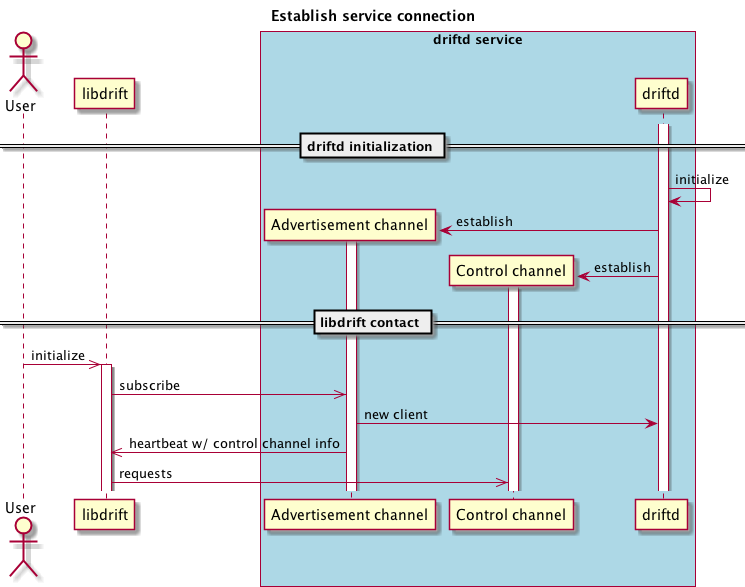
\includegraphics[height=5in]{figs/establish}
  }
  \caption{Using \libdrift to connect to \driftd and perform initial setup.}
\end{figure}


\begin{figure}
  \centering{
    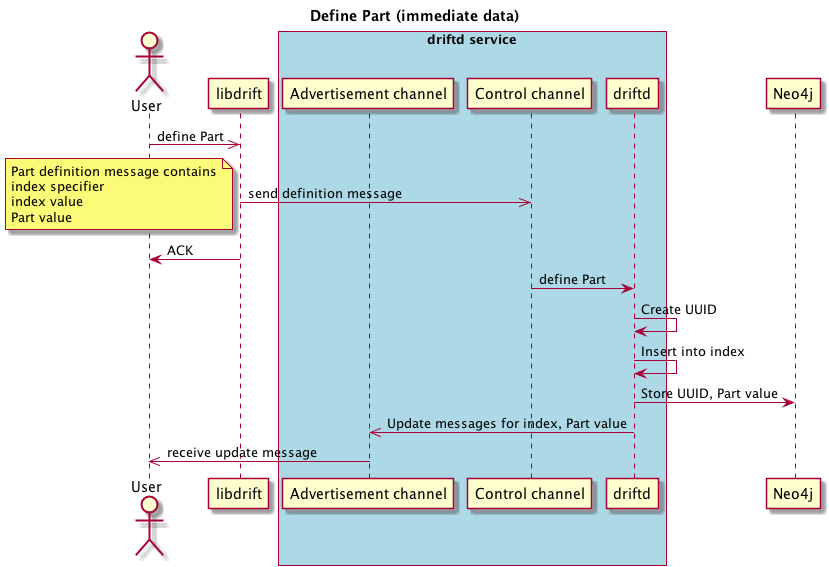
\includegraphics[height=5in]{figs/defining1}
  }
  \caption{Using \libdrift to define a \dpart that contains immediate data.}
\end{figure}



\begin{figure}
  \centering{
    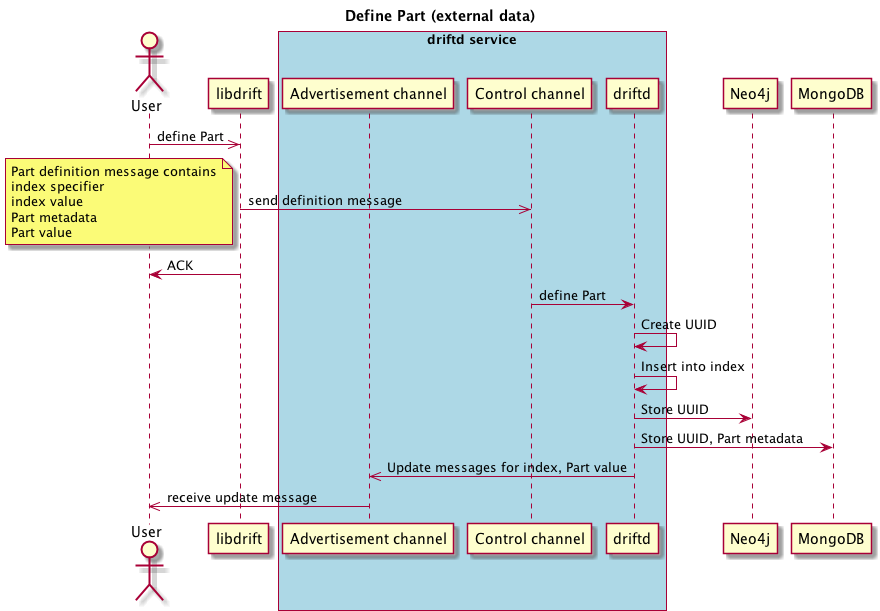
\includegraphics[height=5in]{figs/defining2}
  }
  \caption{Using \libdrift to define a \dpart that contains external data.}
\end{figure}



\begin{figure}
  \centering{
    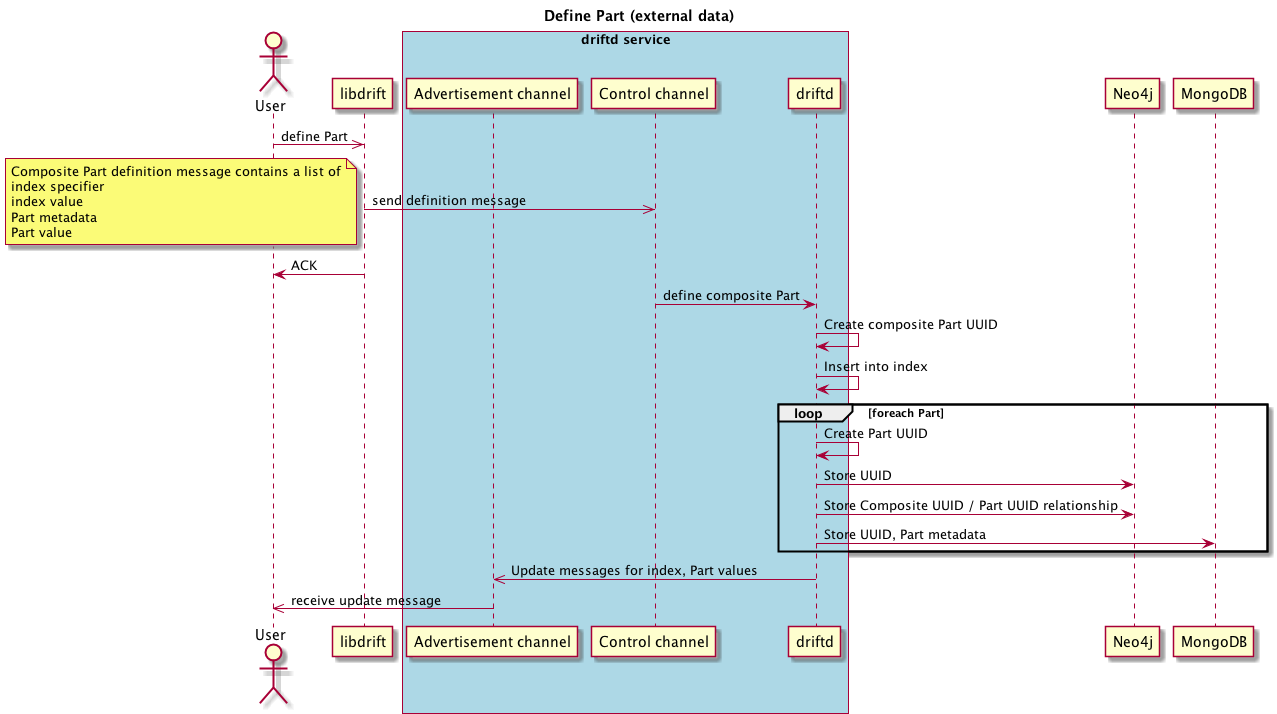
\includegraphics[height=5in]{figs/composite}
  }
  \caption{Using \libdrift to define a composite (fused) \dpart.}

\end{figure}



\begin{figure}
  \centering{
    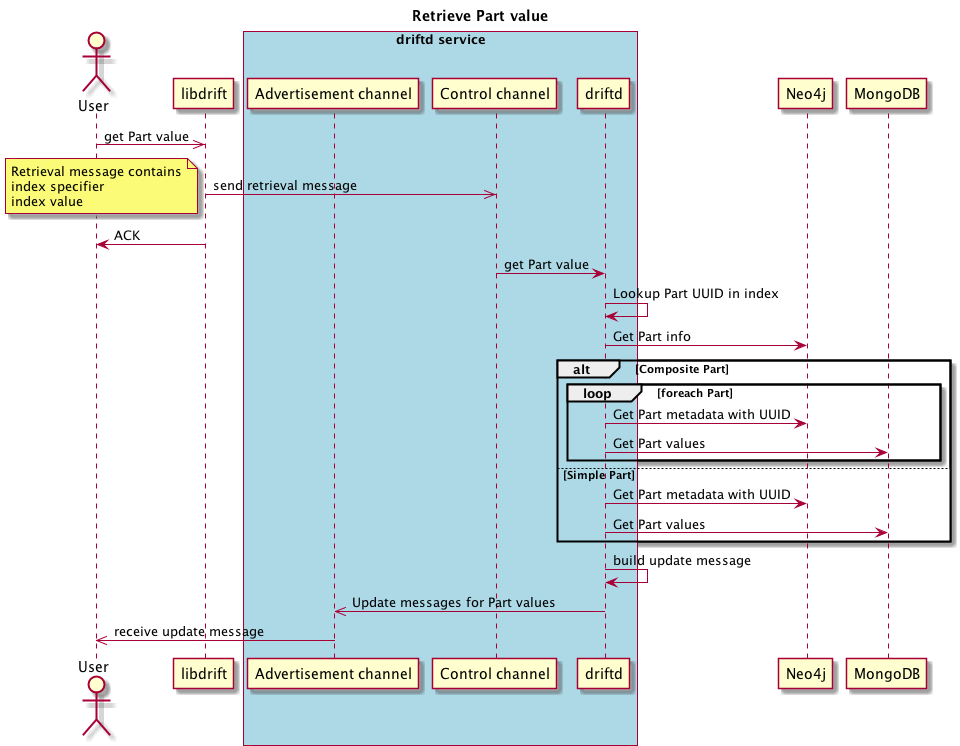
\includegraphics[height=5in]{figs/partvalue}
  }
  \caption{Using \libdrift to retrieve the value of a \dpart.}
\end{figure}







%%% Local Variables: 
%%% mode: latex
%%% TeX-master: "paper"
%%% End: 


    
\section{Extending Drift for enterprise use}
\label{sec:ephemeris}

The effects of ``big data'' problems on information technology organizations have been well-documented.
Whether managing huge online presences, performing large-scale scientific experimentation and simulation,
or ingesting dense streaming data, these organizations face the challenge of converting vast stores of
data to actionable information.  Some of the specific problems faced in the application domain, however,
also manifest themselves in the management of enterprise data stores and sources.  For instance,
computational scientists and enterprise application developers both encounter ``siloed data'', where
domain boundaries restrict awareness about what potentially useful data may exist.
``Write-once-read-never'' issues, where data generation/collection rates outpace analysis and integration
processes, occur in both realms, as simulations generate petabytes of data per day and as documents
relating to design and testing processes accumulate over time, eventually succumbing to bit-rot.

We anticipate the integration of enterprise data stores and sources, once considered the exclusive
province of ``the IT shop'', with data analysis capabilities developed for use in application domains.
An example of this is the mining of employee safety incident data to reveal previously unknown trends and
correlations.  A service-based integration can also provide benefits in the opposite direction.  For
organizations which develop and maintain their own toolsets to support their work processes (such as
software libraries for high-performance computing tasks), making raw and analyzed data outputs available
in regular, extensible, and composable ways can improve productivity, accelerate the solution of new
problems and reduce reinvention of the wheel.

Drift includes specialized low-overhead publish/subscribe interfaces which are necessary for its HPC
role, but are not suitable for enterprise integration.  We are using an Enterprise Service Bus to provide
a service-oriented, discoverable, and general interface to Drift.

\newcommand{\eph}{Drift\xspace}

\begin{figure}
\centering{
  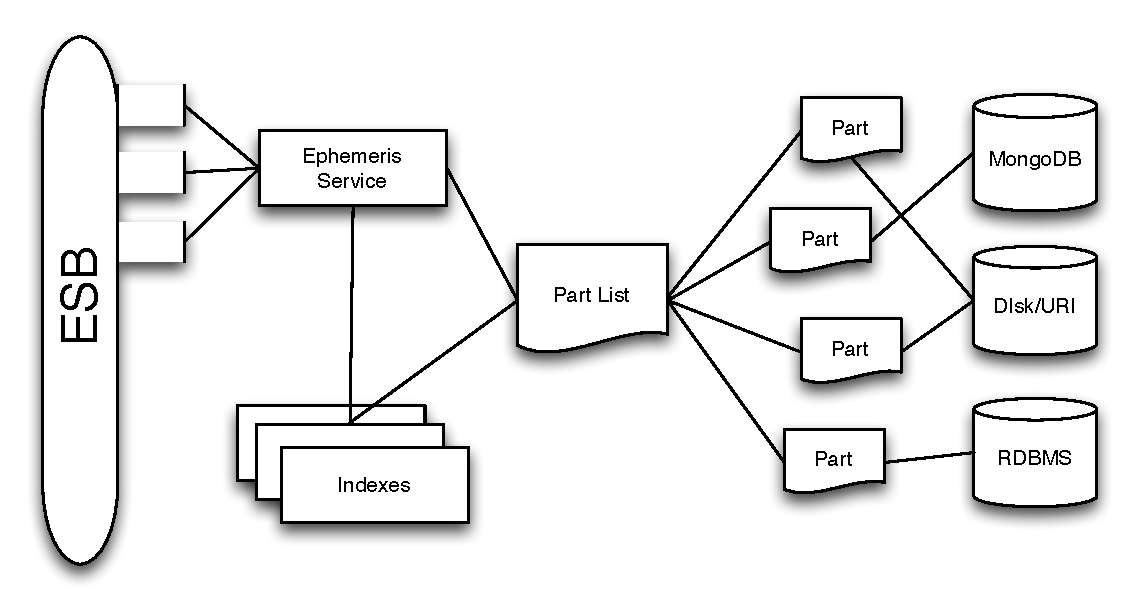
\includegraphics[width=5in]{figs/ep3}
}
\caption{Depiction of system-level relationship between Drift, the ESB, and other ESB services.}
\label{fig:eph}
\end{figure}

\subsection{Enterprise Data Fusion Services}


Drift was originally targeted at HPC and cloud environments, with specialized, low-overhead
publish/subscribe interfaces suited to their requirements.  While those kinds of considerations are
appropriate and necessary in a research software environment, they make integration into larger software
architectures very challenging.  Service-oriented architectures and software-as-a-service models adopted
in the pursuit of enterprise application integration have provided traction on these problems for
business applications.  The growing importance of metadata, Big Data problems, and coupled computations
on heterogeneous platforms is driving the development of research software whose SOA-style encapsulation
promises benefits outside their application domains\textemdash{}if the integration challenges can be
overcome.

We have explored the feasibility of such integration, using the data fusion and flexible indexing
capabilities of Drift as a test case. Our goal is to create an enterprise service with well-defined
endpoints, discovery and introspection capabilities.  We also want to make possible the construction of
more complex service-based offerings which make use of Drift service endpoints.

Given this goal, we have pursued an Enterprise Service Bus (ESB) approach using the open-source Mule
ESB~\cite{mule-esb}, extending Drift as a component called Ephemeris\cite{enterprise14:_patric_m} (Figure~\ref{fig:eph}).  Also, we have built \emph{Connectors} (integration units defined in the Mule
development framework) which will make \eph services available on a deployed Mule ESB.  The Connectors
mediate service requests to a separately running instance using a REST API.  The \eph instance will at
the same time be servicing application clients using its high-performance publish/subscribe interfaces.
In this manner, any service deployed on the ESB will be able to interact with the data fusion facilities
provided by \eph, using fused data defined by applications which have no coupling with the ESB.  This
integration will also provide benefits in the opposite direction: business processes attached to the ESB
will be able to define data fusions which will then be available for \eph application clients.

We have developed a Mule ESB Connector for Neo4j, so that fused data definitions and relationships can be
discovered and examined without interacting with the main service.  We believe this will be a powerful
new capability for integrating application data with enterprise data, making possible more holistic views
of an organization's data environment.  To explore the integration possibilities afforded by Mule's ESB,
we have also developed Connectors for certain internal Sandia services, as well as third-party tools used
internally at Sandia.  A test case for this is the Splunk connector (listing provided as
Appendix~\ref{sec:apx:splunk}.  Using this Connector and the ones provided for Sandia services such as
SAPLE and Drift, a Mule workflow can be constructed which retrieves information on up-to-date operational
information from a Splunk service, queries SAPLE for relevant employee contact information, and stores
the result data in a Drift instance.  Once stored in Drift, the data becomes ``fuse-able'' just as
any other data, providing end users with great flexibility in constructing data types for their own use
that reflect operational data.  



%%% Local Variables: 
%%% mode: latex
%%% TeX-master: "paper"
%%% End: 

    
\section{Conclusion}

Our exploration of data fusion issues with Drift has been illuminating in several respects.  

\begin{itemize}

\item While the Drift software itself has enjoyed limited penetration in the Sandia software development
  community, the ideas behind it still resonate with developers and designers working with diverse data.
  Sandia's Cyber community appears satisfied with the Splunk toolset.  However, Splunk's licensing costs are
  burdensome enough that other domain researchers are starting developments projects, based on
  open-source software, with capability sets similar to both Splunk and Drift.  While the Drift
  implementation may not be ideal infrastructure for all such efforts, there is clearly value in
  establishing this type of software/services layer for use across the Laboratories.

\item A corollary to the previous point is that Laboratory funding for data analytics software should be
  carefully rationalized.  At the beginning of this project, the intended feature set for Drift subsumed
  the capabilities of the Splunk installed base.  12 months later, that situation was dramatically
  reversed, owing entirely to a growing community of Sandians focused on Splunk extension and integration
  development.  Unfortunate timing/coscheduling has been the cause of much unrealized potential in software
  development in large organizations, and part of the research agenda is, and properly, to support
  simultaneous investigation into broad areas (such as software to support data science) in order to gain
  multiple perspectives on large and stubborn issues.  Notwithstanding this, and build-vs-buy
  considerations aside, we believe decisions by the Laboratories to invest large amounts of
  funding (for licensing and development effort) into products like Splunk, creating lock-in engagements
  with software that is itself built from open-source components, should be considered carefully.

\item An ongoing priority for the Laboratories, properly within the purview of the Data Science Research
  Challenge, is to establish procedures for gaining research access to operational data.  In multiple
  instances during this project, goals of the project were significantly impeded by the decision of a
  single individual who happened to be the owner of a particular set of operational data.  No indictment
  of any kind of those individuals is intended here; they are responsible for important components of
  Sandia's operational infrastructure and have acted in good faith with respect to their mission(s).
  However, processes for gaining access to operational data for research purposes should be formalized so
  that they are well-understood and can be applied in an objective manner.  

\end{itemize}

We will be licensing the Drift code as open-source by the end of FY14.  A test suite (including a
document corpus drawn from \cite{govdocs1}) is also planned for inclusion.  Our intention is to explore
future collaborations with university partners that have common interest in the research areas explored
by Drift.  We hope to obtain future funding to continue developing these ideas from the LDRD program,
DOE, or external agencies such as the National Science Foundation.  




%%% Local Variables: 
%%% mode: latex
%%% TeX-master: "paper"
%%% End: 




    % ---------------------------------------------------------------------- %
    % References
    %
    \clearpage
    % If hyperref is included, then \phantomsection is already defined.
    % If not, we need to define it.
    \providecommand*{\phantomsection}{}
    \phantomsection
    \addcontentsline{toc}{chapter}{References}
    \bibliographystyle{plain}
    \bibliography{refs}


    % ---------------------------------------------------------------------- %
    %
    \appendix
    \clearpage
\section*{Appendix}
\subsection*{Sample Mule ESB Cloud Connector}
\label{sec:apx:splunk}

\begin{lstlisting}
/**
 * Sandia Splunk Cloud Connector
 *
 * @author Patrick Widener <patrick.widener@sandia.gov>
 */
@Connector(name="splunk", schemaVersion="0.1", friendlyName="Splunk")
public abstract class SplunkConnector
{
    public static final String BASE_URI = "https://s950881.sandia.gov:8089/";
    

    private HttpClient httpClient;
    
    public SplunkConnector()
    {
	httpClient = new SystemDefaultHttpClient();
	this.setSessionKey(null);
    }
    
    /**
     * Set property
     *
     * @param httpClient
     */
    public void setHttpClient(HttpClient httpClient) { this.httpClient = httpClient; }
    public HttpClient getHttpClient() { return this.httpClient; }
    

    /**
     * Configurable
     */
    @Configurable
    private String splunkUser;

    /**
     * Set property
     * 
     * @param splunkUser
     */
    public void setSplunkUser(String splunkUser) { this.splunkUser = splunkUser; }
    /**
     * Get property
     */
    public String getSplunkUser() { return this.splunkUser; }

    /**
     * Configurable
     */
    @Configurable
    private String splunkPasswd;

    /**
     * Set property
     *
     * @param splunkPasswd
     */
    public void setSplunkPasswd(String splunkPasswd) { this.splunkPasswd = splunkPasswd; }
    /**
     * Get property
     */
    public String getSplunkPasswd() { return this.splunkPasswd; }


    private URIBuilder getUriBuilderBase(String hname) {
	return new URIBuilder().setScheme("https").setHost(hname).setPort(8089);
    }

    /**
     * Connect
     *
     * @param username A username
     * @param password A password
     * @throws ConnectionException
     */
    @Connect
    public void connect(@ConnectionKey String username, String password)
        throws org.mule.api.ConnectionException {
        /*
         * CODE FOR ESTABLISHING A CONNECTION GOES IN HERE
         */

	try {
	    
	    ResponseHandler<String> handler = 
		new ResponseHandler<String>() {
		public String handleResponse(HttpResponse response) throws ClientProtocolException, IOException {
		    HttpEntity e = response.getEntity();
		    if (e != null) {
			return EntityUtils.toString(e);
		    } else {
			return null;
		    }
		}
	    };

	    // Try to copy with Splunk server's self-signed certificate
	    SSLContext sslctx = SSLContext.getInstance("TLS");
	    sslctx.init(null, null, null);
	    SSLSocketFactory sf = new SSLSocketFactory(sslctx, SSLSocketFactory.ALLOW_ALL_HOSTNAME_VERIFIER);
	    Scheme sch = new Scheme("https", 443, sf);
	    getHttpClient().getConnectionManager().getSchemeRegistry().register(sch);

	    URIBuilder b = getUriBuilderBase("s950881.sandia.gov");
	    b.setPath("/servicesNS/admin/search/auth/login");
	    HttpPost httpPost = new HttpPost(b.build());
	    List<NameValuePair> postdata = new ArrayList<NameValuePair>();
	    postdata.add(new BasicNameValuePair("username", getSplunkUser()));
	    postdata.add(new BasicNameValuePair("password", getSplunkPasswd()));
	    postdata.add(new BasicNameValuePair("output_mode", "json"));
	    UrlEncodedFormEntity ure = new UrlEncodedFormEntity(postdata);
	    httpPost.setEntity(ure);

	    String jsonResponse = getHttpClient().execute(httpPost, handler);
	    ObjectMapper jsonMapper = new ObjectMapper();
	    Map<String,String> result = jsonMapper.readValue(jsonResponse, Map.class);
	    this.setSessionKey("Splunk " + result.get("sessionKey"));
	    System.out.println(this.getSessionKey());
	}
	catch (java.lang.Exception X) {
	    System.out.println(X.toString());
	    //	    throw new ConnectionException(ConnectionExceptionCode.INCORRECT_CREDENTIALS, null, "Bye!");
	}
	   

    }

    /**
     * Disconnect
     */
    @Disconnect
    public void disconnect() {
        /*
         * CODE FOR CLOSING A CONNECTION GOES IN HERE
         */
    }

    /**
     * Are we connected
     */
    @ValidateConnection
    public boolean isConnected() {
	if (this.getSessionKey() != null) {
	    return true;
	}
	return false;
    }

    /**
     * Are we connected
     */
    @ConnectionIdentifier
    public String connectionId() {
        return getSessionKey();
    }

    /**
     * Custom processor
     *
     * {@sample.xml ../../../doc/Splunk-connector.xml.sample splunk:my-processor}
     *
     * @param content Content to be processed
     * @return Some string
     */
    @Processor
    public String myProcessor(String content)
    {
        /*
         * MESSAGE PROCESSOR CODE GOES HERE
         */
	System.out.println("in myProcessor, string is " + content);
        return content;
    }


    /**
     * Configurable REST header parameter
     */
    @RestHeaderParam("Authorization")
    private String sessionKey;

    /**
     * Set property
     *
     * @param sessionKey the session key
     */
    public void setSessionKey(String sessionKey) { this.sessionKey = sessionKey; }

    /**
     * Get property
     */
    public String getSessionKey() { return this.sessionKey; }

    
    /**
     * Custom processor
     *
     * {@sample.xml ../../../doc/Splunk-connector.xml.sample splunk:get-results}
     *
     * @param searchId Content to be processed
     * @return Some string
     * @throws java.io.IOException just because
     */
    @Processor
    @RestCall(uri = "https://s950881.sandia.gov:8089/servicesNS/admin/search/search/jobs/?output_mode=json", method = HttpMethod.GET)
    //	      exceptions="{@RestFailOn(expression = "#[header:http.status != 200]")}")
    public abstract String getResults(@RestUriParam("searchId") String searchId) throws java.io.IOException;

    /**
     * GET search/fields
     *
     * Retrieves information about the named field.
     *
     * {@sample.xml ../../../doc/Splunk-connector.xml.sample splunk:get-search-fields}
     *
     * @param fieldName Field to retrieve information for
     * @param outputMode 'json' or 'xml' output format
     * @return XML fragment with field information
     *
     * @throws java.io.IOException For some reason
     */
    @Processor
    @RestCall(uri = BASE_URI + "/servicesNS/admin/search/search/fields/{fieldName}/?output_mode={outputMode}", method = HttpMethod.GET)
    public abstract String getSearchFields(@RestUriParam("fieldName") String fieldName,
					   @Optional @Default("xml") @RestQueryParam("output_mode") String outputMode) throws IOException;

    /**
     * GET search/fields/{field_name}/tags
     *
     * Retrieves tags for the named field.
     *
     * {@sample.xml ../../../doc/Splunk-connector.xml.sample splunk:get-search-fields-tags}
     *
     * @param fieldName Field to retrieve tags
     * @param outputMode 'json' or 'xml' output format
     * @return XML/JSON fragment with field tag information
     *
     * @throws java.io.IOException For some reason
     */
    @Processor
    @RestCall(uri = BASE_URI + "/servicesNS/admin/search/search/fields/{fieldName}/tags/?output_mode={outputMode}", method = HttpMethod.GET)
    public abstract String getSearchFieldsTags(@RestUriParam("fieldName") String fieldName,
					   @Optional @Default("xml") @RestQueryParam("output_mode") String outputMode) throws IOException;


    /**
     * POST search/fields/{field_name}/tags
     *
     * Updates tags for the named field.
     *
     * 
     * {@sample.xml ../../../doc/Splunk-connector.xml.sample splunk:post-search-fields-tags}
     *
     * @param fieldName Field to update tags for
     * @param outputMode 'json' or 'xml' output format
     * @param value Tag name to update for this field
     * @param add Tag to attach to the field_name:value combo
     * @param delete Tag to remove from the field_name:value combo
     * @return XML/JSON fragment with field tag information
     *
     * @throws java.io.IOException For some reason
     */
    @Processor
    @RestCall(uri = BASE_URI + "/servicesNS/admin/search/search/fields/{fieldName}/tags/?output_mode={outputMode}", method = HttpMethod.POST)
    public abstract String postSearchFieldsTags(@RestUriParam("fieldName") String fieldName,
						@RestQueryParam("value") String value,
						@Optional @RestQueryParam("add") String add,
						@Optional @RestQueryParam("delete") String delete,
						@Optional @Default("xml") @RestQueryParam("output_mode") String outputMode) 
	throws IOException;


    /**
     * GET search/tags/{tag_name}
     *
     * Returns a list of field:value pairs associated with tag_name
     *
     * {@sample.xml ../../../doc/Splunk-connector.xml.sample splunk:get-search-tags}
     *
     * @param tagName Name of tag of interest
     * @param outputMode 'json' or 'xml' output format
     * @return XML/JSON fragment with field_name:value pairs
     *
     * @throws java.io.IOException For some reason
     */
    @Processor
    @RestCall(uri = BASE_URI + "/servicesNS/admin/search/search/tags/{tagName}/?output_mode={outputMode}", method = HttpMethod.GET)
    public abstract String getSearchTags(@RestUriParam("tagName") String tagName,
					 @Optional @Default("xml") @RestQueryParam("output_mode") String outputMode) 
	throws IOException;


    /**
     * GET directory
     *
     * Enumerate objects in Splunk.
     *
     * {@sample.xml ../../../doc/Splunk-connector.xml.sample splunk:directory}
     *
     * @param tagName Name of tag of interest
     * @param outputMode 'json' or 'xml' output format
     * @return XML/JSON fragment with field_name:value pairs
     *
     * @throws java.io.IOException For some reason
     */
    @Processor
    @RestCall(uri = BASE_URI + "/servicesNS/admin/search/directory", method = HttpMethod.GET)
    public abstract String directory()
	throws IOException;

}


\end{lstlisting}


    % \printindex

    \begin{SANDdistribution}[NM]% or [CA]
	% \SANDdistCRADA	% If this report is about CRADA work
	% \SANDdistPatent	% If this report has a Patent Caution or Patent Interest
      \SANDdistLDRD	% If this report is about LDRD work

	% External Address Format: {num copies}{Address}
	\SANDdistExternal{}{}
	\bigskip

	% The following MUST BE between the external and internal distributions!
	% \SANDdistClassified % If this report is classified

	% Internal Address Format: {num copies}{Mail stop}{Name}{Org}
	\SANDdistInternal{1}{1319}{Patrick M. Widener}{1423}

	% Mail Channel Address Format: {num copies}{Mail Channel}{Name}{Org}
	%\SANDdistInternalM{}{}{}{}
    \end{SANDdistribution}


    % The second printing
    %\begin{SANDreDistribution}
    %    \SANDdistExternal{}{}
    %    \bigskip
    %    \SANDdistInternal{}{}{}{}
    %    \SANDdistInternalM{}{}{}{}
    %\end{SANDreDistribution}

\end{document}
